\subsection{Activity Diagram}
\vspace{2cm}
\begin{figure}[H]
\centering
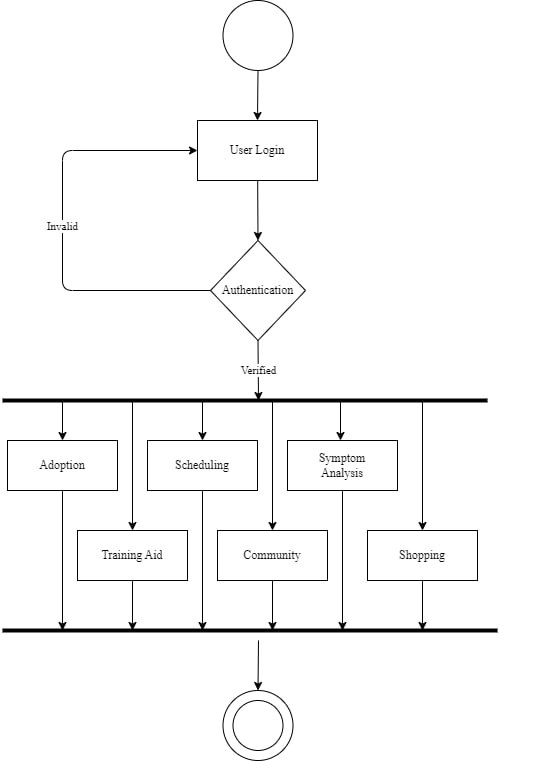
\includegraphics[width=0.9\linewidth]{img/activityU.jpg}
\caption[Activity Diagram from User Perspective]{Activity Diagram from User Perspective}
\label{fig:activity-User}
\end{figure}
\newpage

\noindent\textbf{User Login}\\ The user begins the interaction by initiating the login process. This step involves providing valid credentials, such as a username and password, to gain access to the system.

\noindent\textbf{Authentication}\\Once the user submits login credentials, the system performs authentication to verify the provided information. If the credentials are valid, the user proceeds to the next stage; otherwise, an error message is displayed, prompting the user to re-enter the correct information.

\noindent\textbf{User Activities}\\ After successful authentication, the user gains access to various activities within the system. These activities include:
\begin{itemize}
  \item \textbf{Adoption:} The user can explore and participate in the pet adoption process, connecting with animals in need of loving homes.
  \item \textbf{Scheduling:} The scheduling feature enables users to organize and manage their daily pet-related activities, such as feeding times, veterinary appointments, and other essential tasks.
  \item \textbf{Community:} Users can engage with the community, sharing experiences, seeking advice, and interacting with other pet enthusiasts.
  \item \textbf{Shopping:} The shopping feature allows users to browse, purchase, and manage pet-related products conveniently within the system.
  \item \textbf{Symptom Analysis:} Users can utilize the symptom analysis tool to recognize potential health issues in their pets based on observed symptoms, gaining valuable insights for prompt veterinary attention.
\end{itemize}





\newpage
\vspace{2cm}
\begin{figure}[H]
\centering
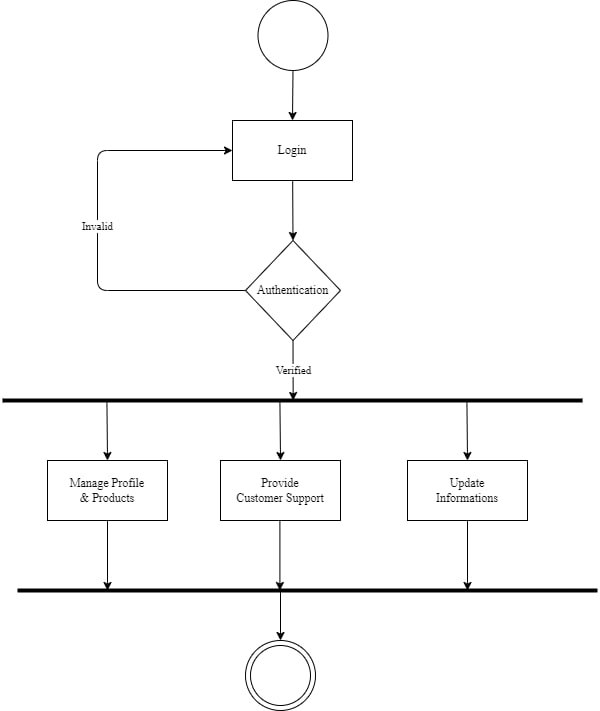
\includegraphics[width=0.9\linewidth]{img/staff.jpg}
\caption[Activity Diagram from Staff Perspective]{Activity Diagram from Staff Perspective}
\label{fig:activity-staff}
\end{figure}

    \noindent\textbf{User Login}\\
        From a staff perspective, the process initiates with user login. Upon receiving user credentials, the system validates the login information. If the provided credentials are valid, the authentication process commences.

        \noindent \textbf{Authentication}\\
        Once the user login is validated, the authentication step ensures the staff member's identity and authorization to access the system. This security measure ensures that only authorized staff members can perform various activities within the system.
  \begin{itemize}
  \item \textbf{Adoption Management:}
        With successful authentication, staff gains access to adoption management functionalities. This feature enables staff to oversee and facilitate the adoption process, ensuring a seamless experience for both potential pet owners and the animals awaiting adoption. Staff can review applications, match pets with suitable owners, and coordinate the adoption process efficiently.

  \item \textbf{Profile and Product Management:}
        The staff's role includes the management of user profiles and products available on the platform. This involves updating and maintaining user information, ensuring accurate records. Additionally, staff can manage the product listings, making sure that the information about available products is current and accurate. This contributes to a well-organized and reliable platform for users.

  \item \textbf{Customer Support:}
        Staff members are equipped to provide customer support as a crucial aspect of user satisfaction. This involves addressing inquiries, resolving issues, and assisting users with any challenges they may encounter. Effective customer support enhances the overall user experience and fosters a positive relationship between the platform and its users.

  \item \textbf{Information Updates:}
        Lastly, staff members have the responsibility of keeping users informed through regular updates. This may include announcements about new features, policy changes, or general information relevant to the user community. Keeping users informed contributes to transparency and user trust in the platform.
\end{itemize}